\documentclass[10pt]{amsart}
\usepackage{amssymb, graphics, bm, verbatim, algorithm2e}

% Use something like:
% % Use something like:
% % Use something like:
% \input{../../macros}

% groupings of objects.
\newcommand{\set}[1]{\left\{ #1 \right\}}
\newcommand{\seq}[1]{\left(#1\right)}
\newcommand{\ang}[1]{\langle#1\rangle}
\newcommand{\tuple}[1]{\left(#1\right)}

% numerical shortcuts.
\newcommand{\abs}[1]{\left| #1\right|}
\newcommand{\floor}[1]{\left\lfloor #1 \right\rfloor}
\newcommand{\ceil}[1]{\left\lceil #1 \right\rceil}

% linear algebra shortcuts.
\newcommand{\change}{\Delta}
\newcommand{\norm}[1]{\left\| #1\right\|}
\newcommand{\dprod}[1]{\langle#1\rangle}
\newcommand{\linspan}[1]{\langle#1\rangle}
\newcommand{\conj}[1]{\overline{#1}}
\newcommand{\gradient}{\nabla}
\newcommand{\der}{\frac{d}{dx}}
\newcommand{\lap}{\Delta}
\newcommand{\kron}{\otimes}
\newcommand{\nperp}{\nvdash}

\newcommand{\mat}[1]{\left( \begin{smallmatrix}#1 \end{smallmatrix} \right)}

% derivatives and limits
\newcommand{\partder}[2]{\frac{\partial #1}{\partial #2}}
\newcommand{\partdern}[3]{\frac{\partial^{#3} #1}{\partial #2^{#3}}}

% Arrows
\newcommand{\diverge}{\nearrow}
\newcommand{\notto}{\nrightarrow}
\newcommand{\up}{\uparrow}
\newcommand{\down}{\downarrow}
% gets and gives are defined!

% ordering operators
\newcommand{\oleq}{\preceq}
\newcommand{\ogeq}{\succeq}

% programming and logic operators
\newcommand{\dfn}{:=}
\newcommand{\assign}{:=}
\newcommand{\co}{\ co\ }
\newcommand{\en}{\ en\ }


% logic operators
\newcommand{\xor}{\oplus}
\newcommand{\Land}{\bigwedge}
\newcommand{\Lor}{\bigvee}
\newcommand{\finish}{$\Box$}
\newcommand{\contra}{\Rightarrow \Leftarrow}
\newcommand{\iseq}{\stackrel{_?}{=}}


% Set theory
\newcommand{\symdiff}{\Delta}
\newcommand{\union}{\cup}
\newcommand{\inters}{\cap}
\newcommand{\Union}{\bigcup}
\newcommand{\Inters}{\bigcap}
\newcommand{\nullSet}{\phi}

% graph theory
\newcommand{\nbd}{\Gamma}

% Script alphabets
% For reals, use \Re

% greek letters
\newcommand{\eps}{\epsilon}
\newcommand{\del}{\delta}
\newcommand{\ga}{\alpha}
\newcommand{\gb}{\beta}
\newcommand{\gd}{\del}
\newcommand{\gf}{\phi}
\newcommand{\gF}{\Phi}
\newcommand{\gl}{\lambda}
\newcommand{\gm}{\mu}
\newcommand{\gn}{\nu}
\newcommand{\gr}{\rho}
\newcommand{\gs}{\sigma}
\newcommand{\gt}{\theta}
\newcommand{\gx}{\xi}

\newcommand{\sw}{\sigma}
\newcommand{\SW}{\Sigma}
\newcommand{\ew}{\lambda}
\newcommand{\EW}{\Lambda}

\newcommand{\Del}{\Delta}
\newcommand{\gD}{\Delta}
\newcommand{\gG}{\Gamma}
\newcommand{\gO}{\Omega}
\newcommand{\gL}{\Lambda}
\newcommand{\gS}{\Sigma}

% Formatting shortcuts
\newcommand{\red}[1]{\textcolor{red}{#1}}
\newcommand{\blue}[1]{\textcolor{blue}{#1}}
\newcommand{\htext}[2]{\texorpdfstring{#1}{#2}}

% Statistics
\newcommand{\distr}{\sim}
\newcommand{\stddev}{\sigma}
\newcommand{\covmatrix}{\Sigma}
\newcommand{\mean}{\mu}
\newcommand{\param}{\gt}
\newcommand{\ftr}{\phi}

% General utility
\newcommand{\todo}[1]{\footnote{TODO: #1}}
\newcommand{\exclaim}[1]{{\textbf{\textit{#1}}}}
\newcommand{\tbc}{[\textbf{Incomplete}]}
\newcommand{\chk}{[\textbf{Check}]}
\newcommand{\oprob}{[\textbf{OP}]:}
\newcommand{\core}[1]{\textbf{Core Idea:}}
\newcommand{\why}{[\textbf{Find proof}]}
\newcommand{\opt}[1]{\textit{#1}}


\DeclareMathOperator*{\argmin}{arg\,min}
\DeclareMathOperator{\rank}{rank}
\newcommand{\redcol}[1]{\textcolor{red}{#1}}
\newcommand{\bluecol}[1]{\textcolor{blue}{#1}}
\newcommand{\greencol}[1]{\textcolor{green}{#1}}


\renewcommand{\~}{\htext{$\sim$}{~}}


% groupings of objects.
\newcommand{\set}[1]{\left\{ #1 \right\}}
\newcommand{\seq}[1]{\left(#1\right)}
\newcommand{\ang}[1]{\langle#1\rangle}
\newcommand{\tuple}[1]{\left(#1\right)}

% numerical shortcuts.
\newcommand{\abs}[1]{\left| #1\right|}
\newcommand{\floor}[1]{\left\lfloor #1 \right\rfloor}
\newcommand{\ceil}[1]{\left\lceil #1 \right\rceil}

% linear algebra shortcuts.
\newcommand{\change}{\Delta}
\newcommand{\norm}[1]{\left\| #1\right\|}
\newcommand{\dprod}[1]{\langle#1\rangle}
\newcommand{\linspan}[1]{\langle#1\rangle}
\newcommand{\conj}[1]{\overline{#1}}
\newcommand{\gradient}{\nabla}
\newcommand{\der}{\frac{d}{dx}}
\newcommand{\lap}{\Delta}
\newcommand{\kron}{\otimes}
\newcommand{\nperp}{\nvdash}

\newcommand{\mat}[1]{\left( \begin{smallmatrix}#1 \end{smallmatrix} \right)}

% derivatives and limits
\newcommand{\partder}[2]{\frac{\partial #1}{\partial #2}}
\newcommand{\partdern}[3]{\frac{\partial^{#3} #1}{\partial #2^{#3}}}

% Arrows
\newcommand{\diverge}{\nearrow}
\newcommand{\notto}{\nrightarrow}
\newcommand{\up}{\uparrow}
\newcommand{\down}{\downarrow}
% gets and gives are defined!

% ordering operators
\newcommand{\oleq}{\preceq}
\newcommand{\ogeq}{\succeq}

% programming and logic operators
\newcommand{\dfn}{:=}
\newcommand{\assign}{:=}
\newcommand{\co}{\ co\ }
\newcommand{\en}{\ en\ }


% logic operators
\newcommand{\xor}{\oplus}
\newcommand{\Land}{\bigwedge}
\newcommand{\Lor}{\bigvee}
\newcommand{\finish}{$\Box$}
\newcommand{\contra}{\Rightarrow \Leftarrow}
\newcommand{\iseq}{\stackrel{_?}{=}}


% Set theory
\newcommand{\symdiff}{\Delta}
\newcommand{\union}{\cup}
\newcommand{\inters}{\cap}
\newcommand{\Union}{\bigcup}
\newcommand{\Inters}{\bigcap}
\newcommand{\nullSet}{\phi}

% graph theory
\newcommand{\nbd}{\Gamma}

% Script alphabets
% For reals, use \Re

% greek letters
\newcommand{\eps}{\epsilon}
\newcommand{\del}{\delta}
\newcommand{\ga}{\alpha}
\newcommand{\gb}{\beta}
\newcommand{\gd}{\del}
\newcommand{\gf}{\phi}
\newcommand{\gF}{\Phi}
\newcommand{\gl}{\lambda}
\newcommand{\gm}{\mu}
\newcommand{\gn}{\nu}
\newcommand{\gr}{\rho}
\newcommand{\gs}{\sigma}
\newcommand{\gt}{\theta}
\newcommand{\gx}{\xi}

\newcommand{\sw}{\sigma}
\newcommand{\SW}{\Sigma}
\newcommand{\ew}{\lambda}
\newcommand{\EW}{\Lambda}

\newcommand{\Del}{\Delta}
\newcommand{\gD}{\Delta}
\newcommand{\gG}{\Gamma}
\newcommand{\gO}{\Omega}
\newcommand{\gL}{\Lambda}
\newcommand{\gS}{\Sigma}

% Formatting shortcuts
\newcommand{\red}[1]{\textcolor{red}{#1}}
\newcommand{\blue}[1]{\textcolor{blue}{#1}}
\newcommand{\htext}[2]{\texorpdfstring{#1}{#2}}

% Statistics
\newcommand{\distr}{\sim}
\newcommand{\stddev}{\sigma}
\newcommand{\covmatrix}{\Sigma}
\newcommand{\mean}{\mu}
\newcommand{\param}{\gt}
\newcommand{\ftr}{\phi}

% General utility
\newcommand{\todo}[1]{\footnote{TODO: #1}}
\newcommand{\exclaim}[1]{{\textbf{\textit{#1}}}}
\newcommand{\tbc}{[\textbf{Incomplete}]}
\newcommand{\chk}{[\textbf{Check}]}
\newcommand{\oprob}{[\textbf{OP}]:}
\newcommand{\core}[1]{\textbf{Core Idea:}}
\newcommand{\why}{[\textbf{Find proof}]}
\newcommand{\opt}[1]{\textit{#1}}


\DeclareMathOperator*{\argmin}{arg\,min}
\DeclareMathOperator{\rank}{rank}
\newcommand{\redcol}[1]{\textcolor{red}{#1}}
\newcommand{\bluecol}[1]{\textcolor{blue}{#1}}
\newcommand{\greencol}[1]{\textcolor{green}{#1}}


\renewcommand{\~}{\htext{$\sim$}{~}}


% groupings of objects.
\newcommand{\set}[1]{\left\{ #1 \right\}}
\newcommand{\seq}[1]{\left(#1\right)}
\newcommand{\ang}[1]{\langle#1\rangle}
\newcommand{\tuple}[1]{\left(#1\right)}

% numerical shortcuts.
\newcommand{\abs}[1]{\left| #1\right|}
\newcommand{\floor}[1]{\left\lfloor #1 \right\rfloor}
\newcommand{\ceil}[1]{\left\lceil #1 \right\rceil}

% linear algebra shortcuts.
\newcommand{\change}{\Delta}
\newcommand{\norm}[1]{\left\| #1\right\|}
\newcommand{\dprod}[1]{\langle#1\rangle}
\newcommand{\linspan}[1]{\langle#1\rangle}
\newcommand{\conj}[1]{\overline{#1}}
\newcommand{\gradient}{\nabla}
\newcommand{\der}{\frac{d}{dx}}
\newcommand{\lap}{\Delta}
\newcommand{\kron}{\otimes}
\newcommand{\nperp}{\nvdash}

\newcommand{\mat}[1]{\left( \begin{smallmatrix}#1 \end{smallmatrix} \right)}

% derivatives and limits
\newcommand{\partder}[2]{\frac{\partial #1}{\partial #2}}
\newcommand{\partdern}[3]{\frac{\partial^{#3} #1}{\partial #2^{#3}}}

% Arrows
\newcommand{\diverge}{\nearrow}
\newcommand{\notto}{\nrightarrow}
\newcommand{\up}{\uparrow}
\newcommand{\down}{\downarrow}
% gets and gives are defined!

% ordering operators
\newcommand{\oleq}{\preceq}
\newcommand{\ogeq}{\succeq}

% programming and logic operators
\newcommand{\dfn}{:=}
\newcommand{\assign}{:=}
\newcommand{\co}{\ co\ }
\newcommand{\en}{\ en\ }


% logic operators
\newcommand{\xor}{\oplus}
\newcommand{\Land}{\bigwedge}
\newcommand{\Lor}{\bigvee}
\newcommand{\finish}{$\Box$}
\newcommand{\contra}{\Rightarrow \Leftarrow}
\newcommand{\iseq}{\stackrel{_?}{=}}


% Set theory
\newcommand{\symdiff}{\Delta}
\newcommand{\union}{\cup}
\newcommand{\inters}{\cap}
\newcommand{\Union}{\bigcup}
\newcommand{\Inters}{\bigcap}
\newcommand{\nullSet}{\phi}

% graph theory
\newcommand{\nbd}{\Gamma}

% Script alphabets
% For reals, use \Re

% greek letters
\newcommand{\eps}{\epsilon}
\newcommand{\del}{\delta}
\newcommand{\ga}{\alpha}
\newcommand{\gb}{\beta}
\newcommand{\gd}{\del}
\newcommand{\gf}{\phi}
\newcommand{\gF}{\Phi}
\newcommand{\gl}{\lambda}
\newcommand{\gm}{\mu}
\newcommand{\gn}{\nu}
\newcommand{\gr}{\rho}
\newcommand{\gs}{\sigma}
\newcommand{\gt}{\theta}
\newcommand{\gx}{\xi}

\newcommand{\sw}{\sigma}
\newcommand{\SW}{\Sigma}
\newcommand{\ew}{\lambda}
\newcommand{\EW}{\Lambda}

\newcommand{\Del}{\Delta}
\newcommand{\gD}{\Delta}
\newcommand{\gG}{\Gamma}
\newcommand{\gO}{\Omega}
\newcommand{\gL}{\Lambda}
\newcommand{\gS}{\Sigma}

% Formatting shortcuts
\newcommand{\red}[1]{\textcolor{red}{#1}}
\newcommand{\blue}[1]{\textcolor{blue}{#1}}
\newcommand{\htext}[2]{\texorpdfstring{#1}{#2}}

% Statistics
\newcommand{\distr}{\sim}
\newcommand{\stddev}{\sigma}
\newcommand{\covmatrix}{\Sigma}
\newcommand{\mean}{\mu}
\newcommand{\param}{\gt}
\newcommand{\ftr}{\phi}

% General utility
\newcommand{\todo}[1]{\footnote{TODO: #1}}
\newcommand{\exclaim}[1]{{\textbf{\textit{#1}}}}
\newcommand{\tbc}{[\textbf{Incomplete}]}
\newcommand{\chk}{[\textbf{Check}]}
\newcommand{\oprob}{[\textbf{OP}]:}
\newcommand{\core}[1]{\textbf{Core Idea:}}
\newcommand{\why}{[\textbf{Find proof}]}
\newcommand{\opt}[1]{\textit{#1}}


\DeclareMathOperator*{\argmin}{arg\,min}
\DeclareMathOperator{\rank}{rank}
\newcommand{\redcol}[1]{\textcolor{red}{#1}}
\newcommand{\bluecol}[1]{\textcolor{blue}{#1}}
\newcommand{\greencol}[1]{\textcolor{green}{#1}}


\renewcommand{\~}{\htext{$\sim$}{~}}


% Use something like:
% % Use something like:
% % Use something like:
% \input{../../amsartMacros}

\newtheorem{thm}{Theorem}[subsection]
\newtheorem{cor}[thm]{Corollary}
\newtheorem{lem}[thm]{Lemma}
\newtheorem{fact}[thm]{Fact}
\newtheorem{claim}[thm]{Claim}

\newtheorem{assumption}[thm]{Assumption}

\newtheorem{defn}[thm]{Definition}

\theoremstyle{remark}
\newtheorem{alg}[thm]{Algorithm}
\newtheorem*{notation}{Notation}
\newtheorem*{rem}{Remark}
\newtheorem*{hint}{Hint}
\newtheorem*{ack}{Acknowledgement}

\newtheorem{question}[thm]{Question}
\newtheorem{answer}[thm]{Answer}


\newtheorem{thm}{Theorem}[subsection]
\newtheorem{cor}[thm]{Corollary}
\newtheorem{lem}[thm]{Lemma}
\newtheorem{fact}[thm]{Fact}
\newtheorem{claim}[thm]{Claim}

\newtheorem{assumption}[thm]{Assumption}

\newtheorem{defn}[thm]{Definition}

\theoremstyle{remark}
\newtheorem{alg}[thm]{Algorithm}
\newtheorem*{notation}{Notation}
\newtheorem*{rem}{Remark}
\newtheorem*{hint}{Hint}
\newtheorem*{ack}{Acknowledgement}

\newtheorem{question}[thm]{Question}
\newtheorem{answer}[thm]{Answer}


\newtheorem{thm}{Theorem}[subsection]
\newtheorem{cor}[thm]{Corollary}
\newtheorem{lem}[thm]{Lemma}
\newtheorem{fact}[thm]{Fact}
\newtheorem{claim}[thm]{Claim}

\newtheorem{assumption}[thm]{Assumption}

\newtheorem{defn}[thm]{Definition}

\theoremstyle{remark}
\newtheorem{alg}[thm]{Algorithm}
\newtheorem*{notation}{Notation}
\newtheorem*{rem}{Remark}
\newtheorem*{hint}{Hint}
\newtheorem*{ack}{Acknowledgement}

\newtheorem{question}[thm]{Question}
\newtheorem{answer}[thm]{Answer}


%opening
\title{Linear Algebra: Answer to Homework 8}
\author{vishvAs vAsuki}

\begin{document}

\maketitle

\section{25.1}
\subsection{a}
\begin{thm}
A is Tridiagonal. $A=A^{*}$. All sub and super diagonal entries are non zero. All ew of A are distinct.
\end{thm}
\begin{proof}
Suppose that for any l, $A-lI$ has rank $\geq m-1$. (This is shown in the lemma below.)

Let $l_{i}$ be an ew of A. Then, $dim(A-l_{i}I) \geq m-1$. But, we know that $(A-l_{i}I) \perp rowspace(A-l_{i}I)$, and that $dim(A-l_{i}I) + rank(A-l_{i}I) = m$. So, $dim(A-l_{i}I) \leq m-1$. Thus, $dim(A-l_{i}I) = m-1$ and $dim(Null(A-l_{i}I)) = 1$.

Thus, there are m eigenspaces, each of dimension 1. Thus, there are m distinct eigenvalues.
\end{proof}

\begin{lem}
A is Tridiagonal. $A=A^{*}$. All sub and super diagonal entries are non zero. For any l, $A-lI$ has rank $\geq m-1$.
\end{lem}
\begin{proof}
As $A=A^{*}$, A is unitarily diagonalizable, and its SVD is same as its eigenvalue decomposition. Similar is the case with $B = A-lI$. \tbc
\end{proof}


\subsection{b}
A is upper Hessenberg. All its subdiagonal entries are nonzero. Then the following example shows that the eigenvalues of A are not necessarily distinct.

$B = \mat{3 & 0  \\  1 & 3 }$.

\section{27.2}
\begin{defn}
$A\in C^{m\times m}$ is arbitrary. The set of all Rayleigh quotients of A corresponding to all nonzero vectors $x\in C^{m}$ is the field of values, or the numerical range of A, a subset  of the complex plane denoted by W(A).
\end{defn}

\begin{notation}
$l_{i}$ represents the ew of A. $v_{i}$ represents the corresponding ev. L(A) represents the spectrum of A.
\end{notation}

\subsection{a}
\begin{thm}
W(A) contains the convex hull of the ew's of A.
\end{thm}
\begin{proof}
$\frac{v_{i}^{*}Av_{i}}{v_{i}^{*}v_{i}} = l_{i}$. So, all $l_{i}$ is in W(A). By a well known theorem, W(A) is convex. So, all $\sum^{i} w_{i}l_{i} : \sum_{i}w_{i} = 1$ is in W(A).
\end{proof}

\subsection{b}
\begin{thm}
If A is normal, W(A) = convex hull of the ew's of A.
\end{thm}
\begin{proof}
As A is normal, it is unitarily diagonalizable: $A=Q^{*}LQ$. So, let $v_{1}, .. v_{m}$ be its orthogonal ev's. These span the entire space. Then, any $x = \sum t_{i}v_{i}$.

$\frac{x^{*}Ax}{x^{*}x} = \frac{(\sum_{i} t_{i}v_{i}^{*})A(\sum_{i} t_{i}v_{i})}{(\sum_{i} t_{i}v_{i}^{*})(\sum_{i} t_{i}v_{i})} = \frac{(\sum_{i} t_{i}v_{i}^{*})(\sum_{i} t_{i}l_{i}v_{i})}{(\sum_{i} t_{i}v_{i}^{*})(\sum_{i} t_{i}v_{i})} = \sum_{i} l_{i}\frac{t_{i}^{2}}{\sum_{i} t_{i}^{2}}$. Writing $\frac{t_{i}^{2}}{\sum_{i} t_{i}^{2}} = w_{i}$, we get $\frac{x^{*}Ax}{x^{*}x} = \sum_{i} l_{i}w_{i}$. Also, we see that $\sum_{i}w_{i} = 1$. So, any $\frac{x^{*}Ax}{x^{*}x}$ is in the convex hull of L(A).

We know from an earlier theorem that the convex hull of L(A) is always contained in W(A).

So, W(A) = the convex hull of L(A).
\end{proof}

\section{30.7}
Make a random real symmetric tridiagonal matrix T of dimension 100.
Find its eigenvalue decomposition: $T=QDQ^{T}$. Plot a few of the ev on a log scale (abs values of a few columns of Q) and observe the phenomenon of localization. What part of the 10000 entries of Q are greater than $10^{-10}$ in magnitude? What is the answer if instead of a random matrix, T is a discrete Laplacian with entries 1, -2, 1.

\subsection{Solution}
In the graph below, we clearly observe, what may be called, the phenomenon of localization.

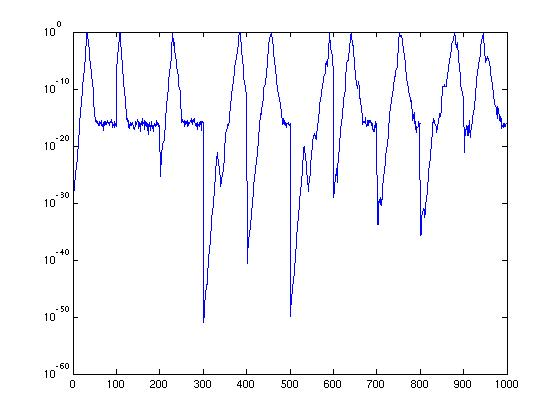
\includegraphics{eigenvectorLocality.jpg}

For a random T, 5564 of the 10000 entries of Q were $\leq 10^{-10}$ in magnitude, the rest 4436 were above $10^{-10}$.

For the discrete Laplacian, 0 entries of Q were $\leq 10^{-10}$ in magnitude, the rest 10000 were above $10^{-10}$.

\section{}
Generate a random $50\times 50$ tridiagonal matrix in Matlab, after setting the seed to be 1 i.e. type ``rand('seed',1);''. Compute its eigenvalues using the ``eig'' command in Matlab. Consider the smallest eigenvalue in magnitude and use following strategies to compute the corresponding eigenvector:
  \begin{enumerate}
  \item Fix the first component of the eigenvector to be $1$ and then solve for the remaining components of the eigenvector.
  \item Fix the last component of the eigenvector to be $1$ and then solve for the remaining components of the eigenvector.
  \end{enumerate}

Compare the obtained eigenvector by each of the above strategies with the one generated by Matlab.

Is any of the eigenvectors obtained by the above given strategies close to the actual eigenvector (one generated by Matlab)? If not, what can be a possible justification?

\subsection{Answer}
The code will be emailed to the TA.

We are interested in comparing the directions of the eigenvectors obtained by either of these strategies with the direction of the eigenvector obtained using Matlab.

This was done by looking at the absolute value of the inner product of the normalized vectors. In both cases, this value beautifully turns out to be 1; which is as expected.

Any initial appearence of difference between the eivenvectors may be explained by the lack of normalization and change in signs.

Incidentally, the veracity of the eigenvectors obtained was verified by checking that $\norm{Ax-lx} = O(\eps)$.

\section{}
\begin{thm}
Let $A$ be $m\times n$ and $B$ be $n\times m$. Then, the matrices $U = \mat{AB&0\\B&0}$ and $V = \mat{0&0\\B&BA}$ have the same eigenvalues. 
\end{thm}
\begin{proof}
Take $X = \mat{I & A\\ I & I}$. Note that X is invertible. We see that UX=XV. So, V can be obtained by a similarity transformation of U. So, they have the same eigenvalues.
\end{proof}

\section{}
Give the eigenvalue decompositions and Schur 
    decompositions of the following matreces.

\begin{notation}
The eigenvalue decomposition is $S^{-1}LS$. The schur decomposition is $Q^{*}TQ$.
\end{notation}
$$
    A = \mat{0 & 1  \\  1 & 0 }
$$

\begin{verbatim}
S =

   -0.7071    0.7071
    0.7071    0.7071


L =

    -1     0
     0     1

Q =

   -0.7071    0.7071
    0.7071    0.7071


U =

    -1     0
     0     1

\end{verbatim}

$$
    B = \mat{0 & 0  \\  1 & 0 }
$$
\begin{verbatim}
S =

         0    0.0000
    1.0000   -1.0000


L =

     0     0
     0     0


Q =

     0    -1
     1     0


U =

     0    -1
     0     0
\end{verbatim}


$$
    C = \mat{5 & -3 \\ -1 & 3 }
$$
\begin{verbatim}
S =

    0.9487    0.7071
   -0.3162    0.7071


L =
     6     0
     0     2


Q =

    0.9487    0.3162
   -0.3162    0.9487


U =

     6    -2
     0     2
\end{verbatim}

% 
% \bibliographystyle{plain}
% \bibliography{../linAlg}

\end{document}

